% This is samplepaper.tex, a sample chapter demonstrating the
% LLNCS macro package for Springer Computer Science proceedings;
% Version 2.20 of 2017/10/04
%
\documentclass[runningheads]{llncs}
%
% Used for displaying a sample figure. If possible, figure files should
% be included in EPS format.
%
% If you use the hyperref package, please uncomment the following line
% to display URLs in blue roman font according to Springer's eBook style:
% \renewcommand\UrlFont{\color{blue}\rmfamily}





\usepackage{amsmath}
\usepackage{amssymb}
\usepackage{todonotes}
\usepackage{stmaryrd}
\usepackage{xspace}
\usepackage{listings}
\usepackage{comment}
\usepackage{mathtools}
%\usepackage[all]{xy}
\usepackage{tikz}
\usetikzlibrary{trees}
\usepackage{multirow}
\usepackage{array}
\usepackage{graphics}
\usepackage[cmtip,all]{xy}
\usepackage{units}

%\xymatrix@C-=0.5cm

\newcommand{\longsquiggly}{\xymatrix@C-=0.5cm{{}\ar@{~>}[r]&{}}}

\newcommand{\todonote}[1]{\todo[inline, color=blue!20]{\textbf{TODO:} #1}}
\newcommand{\sectionword}{section}
\newcommand{\appendixword}{appendix}
\newcommand{\figureword}{Fig.}
\newcommand{\eqdef}{\overset{\mathrm{def}}{=}}
\newcommand{\ruleno}[1]{\mbox{[\textsc{#1}]}}
\newcommand{\bigslant}[2]{{\raisebox{.2em}{$#1$}\left/\raisebox{-.2em}{$#2$}\right.}}
\newcommand{\lowupbound}[2]{\;\; \overset{\makebox[0pt]{\mbox{\normalfont\tiny {C = $#2$}}}}{ \underset{\makebox[0pt]{\mbox{\normalfont\tiny {C = $#1$}}}}{\gtrless}} \;\;}
\newcommand{\argmax}[1]{\underset{\makebox[0pt]{\mbox{\normalfont\tiny {$#1$}}}}{argmax} \;\;}
\newcommand{\maxd}{\max^{\bullet}}
\let\emptyset\varnothing

\newcommand{\grterms}{\mathcal{T}_{\emptyset}}
\newcommand{\Dom}{\mathcal{D}om}
\newcommand{\VRan}{\mathcal{VR}an}

\newcommand{\substitute}[3]{#1\,[\bigslant{#2}{#3}]}
\newcommand{\substupd}[3]{#1[#2 \mapsto #3]}

\newcommand{\taskst}[2]{\langle #1 ,\, #2 \rangle}
\newcommand{\mkenv}[2]{(#1 ,\, #2)}
\newcommand{\unigoal}[2]{#1 \equiv #2}
\newcommand{\conjgoal}[2]{#1 \land #2}
\newcommand{\disjgoal}[2]{#1 \lor #2}
\newcommand{\freshgoal}[2]{\texttt{\underline {fresh}} \, #1\;.\; #2}
\newcommand{\invokegoal}[3]{#1\,(#2, \, \dots, \, #3)}
\newcommand{\einit}{e_{init}}
\newcommand{\ninit}{n_{init}}

\newcommand{\schemetrans}[6]{\withenv{#2,\,#3,\,#4,\,#5}{#1} \longsquiggly #6}
\newcommand{\schemewithvset}[2]{{#1}^{#2}}

\newcommand{\schemenode}[1]{
\begin{tikzpicture}[sibling distance=3cm,edge from parent/.style={draw,-latex}]
  \node[rectangle,draw]{#1};
\end{tikzpicture}
 }

\newcommand{\schemesarrow}[3]{
\begin{tikzpicture}[sibling distance=3cm,edge from parent/.style={draw,-latex}]
  \node[rectangle,draw]{#1}child {node[circle,draw]{#3}edge from parent node[right]{\tiny{#2}}};
\end{tikzpicture}}

\newcommand{\schemedarrow}[3]{
\begin{tikzpicture}[sibling distance=3cm,edge from parent/.style={draw,-latex}]
  \node[rectangle,draw]{#1}child {node[circle,draw]{#3}edge from parent node[right]{\tiny{#2}}};
\end{tikzpicture}}

\newcommand{\schemefork}[2]{
  \begin{tikzpicture}[edge from parent/.style={draw,-latex}]
   \coordinate   
      child {node[circle,draw]{#1}}
      child {node[circle,draw]{#2}} ;
\end{tikzpicture}}

\newcommand{\upd}[2]{\mbox{\textbf{upd}}\,(#1,\, #2)}
\newcommand{\constr}[2]{\mbox{\textbf{constr}}\,(#1,\, #2)}

%\newcommand{\schemefork}[2]{\begin{array}{cccc} & \swarrow & \searrow \\ #1 & & & #2 \end{array}}

\newcommand{\withenv}[2]{\left< #1 \right> \;\vdash\; #2}
\newcommand{\onepremrule}[2]{\dfrac{#1}{#2}}
\newcommand{\twopremrule}[3]{\dfrac{#1,\; #2}{#3}}
\newcommand{\threepremrule}[4]{\dfrac{#1,\;  #2,\;  #3}{#4}}

\newcommand{\lazystream}[1]{\texttt{Lazy [{#1}]}}
\newcommand{\consstream}[2]{\texttt{Cons #1 [{#2}]}}

\newcommand{\sembr}[1]{\llbracket #1 \rrbracket}
\newcommand{\tra}[1]{\mathcal{T}r^{ans}(#1)}
\newcommand{\trs}[1]{\mathcal{T}r^{st}(#1)}

\newcommand{\mK}{\textsc{miniKanren}\xspace}

\newcommand{\costdisj}[2]{cost_{\oplus}(#1 \oplus #2)}
\newcommand{\costconj}[2]{cost_{\otimes}(#1 \otimes #2)}
\newcommand{\lookuptime}[1]{\texttt{lookup}\,(#1)}
\newcommand{\addtime}[1]{\texttt{add}\,(#1)}
\renewcommand{\O}{\mathcal{O}}


%% Listings

\lstdefinelanguage{minikanren}{
keywords={fresh},
sensitive=true,
commentstyle=\small\itshape\ttfamily,
keywordstyle=\textbf,
identifierstyle=\ttfamily,
basewidth={0.5em,0.5em},
columns=fixed,
fontadjust=true,
literate={fun}{{$\lambda\;\;$}}1 {->}{{$\to$}}3 {===}{{$\,\equiv\,$}}1 {=/=}{{$\not\equiv$}}1 {|>}{{$\triangleright$}}3 {/\\}{{$\wedge$}}2 {\\/}{{$\vee$}}2,
morecomment=[s]{(*}{*)}
}

\lstset{
mathescape=true,
language=minikanren
}

\usepackage{letltxmacro}
\newcommand*{\SavedLstInline}{}
\LetLtxMacro\SavedLstInline\lstinline
\DeclareRobustCommand*{\lstinline}{%
  \ifmmode
    \let\SavedBGroup\bgroup
    \def\bgroup{%
      \let\bgroup\SavedBGroup
      \hbox\bgroup
    }%
  \fi
  \SavedLstInline
}


%%
%% end of the preamble, start of the body of the document source.
\begin{document}

%%
%% The "title" command has an optional parameter,
%% allowing the author to define a "short title" to be used in page headers.
\title{Scheduling Complexity of Interleaving Search}

\author{Anonymous author(s)}
%
\authorrunning{Anonymous author(s)}
% First names are abbreviated in the running head.
% If there are more than two authors, 'et al.' is used.
%
\institute{Anonymous institute(s)}

%%
%% This command processes the author and affiliation and title
%% information and builds the first part of the formatted document.
\maketitle

%%
%% The abstract is a short summary of the work to be presented in the
%% article.
\begin{abstract}
  We study the worst-case time complexity of relational programs for the canonical implementation of \mK. We propose a model that breaks the evaluation time in \mK into
  several different parts and provides methods to estimate the complexity of these parts. These methods can be combined into an approach for
  analyzing the complexity of recursive relations using the ideas originating from symbolic execution. Our approach puts a number of limitations
  on the program being analyzed but we show that is still practically applicable by applying it to a number of typical relations in \mK.
  
\keywords{miniKanren, interleaving search, time complexity, symbolic execution}
\end{abstract}


% \section{Introduction}
\label{sec:intro}

\colorbox{red!20}{\textbf{Motivational example:}}
\begin{lstlisting}[basicstyle=\small]
   append$^o_{naive}$ = fun a b ab ->
     ((a === Nil) /\ (ab === b)) \/
     (fresh (h t tb)
        (a === Cons(h, t)) /\
        (append$^o_{naive}$ t b tb) /\
        (ab === Cons(h, tb)) 
     )
\end{lstlisting}

\begin{lstlisting}[basicstyle=\small]
   append$^o_{opt}$ = fun a b ab ->
     ((a === Nil) /\ (ab === b)) \/
     (fresh (h t tb)
        (a === Cons(h, t)) /\
        (ab === Cons(h, tb) /\
        (append$^o_{opt}$ t b tb)) 
     )
\end{lstlisting}

\colorbox{red!20}{\parbox{\textwidth}{\textbf{State requirements for our method (informally)}}}

We prove the theorem only for goals in DNF.

\[
\begin{array}{lcl}
B_{nf} & = &  \unigoal{\mathcal{T}_\mathcal{X}}{\mathcal{T}_\mathcal{X}} \; \mid \;
                     \invokegoal{R^k}{\mathcal{T}_\mathcal{X}}{\mathcal{T}_\mathcal{X}} \\
C_{nf} & = & B_{nf} \; \mid \; \conjgoal{C_{nf}}{B_{nf}} \\
F_{nf} & = & C_{nf} \; \mid \; \freshgoal{X}{F_{nf} } \\
D_{nf} & = & F_{nf} \; \mid \; \disjgoal{D_{nf}}{F_{nf}}
\end{array}
\]

We also have a requirement that all recursive calls performed during unification are \emph{grounding} and \emph{non-repetitive}.

\begin{definition}
  We call relational invocation
  
  \[\taskst{\invokegoal{R^k}{t_1}{t_k}}{e}\]

  \emph{grounding} and \emph{non-repetitive} if 

  \[ \forall (\sigma^{a}, n^{a}) \in \tra{\taskst{\invokegoal{R^k}{t_1}{t_k}}{e}} \,:\, FV(t_i \sigma^{a}) = \emptyset \]

  and
  
  \[ \forall (\sigma_1^{a},\, n_1^{a}),\, (\sigma_2^{a},\, n_2^{a}) \in \tra{\taskst{\invokegoal{R^k}{t_1}{t_k}}{e}} \,:\, (t_1 \sigma_1^{a}, \dots, t_k \sigma_1^{a}) \ne (t_1 \sigma_2^{a},\, \dots, t_k \sigma_2^{a}) \]
\end{definition}


\section{Background: syntax and operational semantics}
\label{sec:background}

\colorbox{red!20}{\parbox{\textwidth}{General description of \mK as embedded language based on lazy streams}}

In this section, we recollect some known formal descriptions for \mK language that will be used as a basis for our development.
Specifically, we restate the syntax of the basic version of the language and the operational semantics for program evaluation.
The descriptions here are taken from~\cite{CertifiedSemantics} (with a few non-essential adjustments for presentation purposes) to make
the paper self-contained, more details and explanations can be found there.

\begin{figure}[t]
\centering
\[
\begin{array}{ccll}
  \mathcal{C} & = & \{C_i^{k_i}\} & \mbox{constructors} \\
  \mathcal{T}_X & = & X \cup \{C_i^{k_i} (t_1, \dots, t_{k_i}) \mid t_j\in\mathcal{T}_X\} & \mbox{terms over the set of variables $X$} \\
  \mathcal{D} & = & \mathcal{T}_\emptyset & \mbox{ground terms}\\
  \mathcal{X} & = & \{ x, y, z, \dots \} & \mbox{syntactic variables} \\
  \mathcal{A} & = & \{ x^?, y^?, z^? \dots \} & \mbox{logic variables} \\
  \mathcal{R} & = & \{ R_i^{k_i}\} &\mbox{relational symbols with arities} \\[2mm]
  \mathcal{G} & = & \mathcal{T_X}\equiv\mathcal{T_X}   &  \mbox{equality} \\
              &   & \mathcal{G}\wedge\mathcal{G}     & \mbox{conjunction} \\
              &   & \mathcal{G}\vee\mathcal{G}       &\mbox{disjunction} \\
              &   & \mbox{\lstinline|fresh|}\;\mathcal{X}\;.\;\mathcal{G} & \mbox{fresh variable introduction} \\
              &   & R_i^{k_i} (t_1,\dots,t_{k_i}),\;t_j\in\mathcal{T_X} & \mbox{relational symbol invocation} \\[2mm]
  \mathcal{S} & = & \{R_i^{k_i} = \lambda\;x_1^i\dots x_{k_i}^i\,.\, g_i;\}\; g & \mbox{specification}
\end{array}
\]
\caption{The syntax of \mK}
\label{fig:syntax}
\end{figure}

The syntax of the basic version of \mK is shown in Fig.~\ref{fig:syntax}. 
All data is presented using terms $\mathcal{T}_X$ built from a fixed set of constructors $\mathcal{C}$ with known arities and variables
from a given set $X$.
We parameterize the terms with an alphabet of variables since in the semantic description we will need \emph{two} kinds of variables:
\emph{syntactic} variables $\mathcal{X}$, used for bindings in the definitions, and \emph{logic} variables $\mathcal{A}$, which are
introduced and unified during the evaluation.

In this version of \mK there are five types of goals: unification of two terms, conjunction and disjunction of goals (the
``\lstinline|conde|'' operator from the canonical versions of \mK, split in the two for simplicity), fresh logic variable introduction, and
invocation of some relational definition. For the sake of brevity, in code snippets, we abbreviate immediately nested ``\lstinline|fresh|''
constructs into the one, writing ``\lstinline|fresh $x$ $y$ $\dots$ . $g$|'' instead of
``\lstinline|fresh $x$ . fresh $y$ . $\dots$ $g$|''.

The \emph{specification} $\mathcal{S}$ consists of a set of relational definitions and a top-level goal.
A top-level goal represents a search procedure that returns a stream of substitutions for the free variables of the goal.
The language we consider is first-order, as goals can not be passed as parameters, returned, or constructed at runtime.

During the evaluation of \mK program an environment, consisting of substitution for logic variables and a counter of allocated logic
variables, is threaded through the computation and updated in every unification and fresh variable introduction.
The substitution in the environment at a given point and a given branch of evaluation contains all the information about relations between
the logical variables at this point. We will later refer to the substitution in the environment at a given point as a ``current substitution''
in informal explanations.
The different branches are combined via \emph{interleaving search} procedure~\cite{InterleavingSearch}.
The answers for the given query are extracted from the final environments (they are the values of the queried variables in the substitution
in the final environment).

This search procedure is formally described by operational semantics in the form of a labeled transition system.
This semantics corresponds to the canonical implementation of interleaving search. 

\begin{figure}[t]
\centering
\[
\begin{array}{ccllcccll}
  \Sigma & = & \mathcal{A} \to \mathcal{T}_\mathcal{A} & \mbox{substitutions} &\qquad\qquad&        S & = & \taskst{\mathcal{G}}{E} & \mbox{task} \\
       E & = & \Sigma \times \mathbb{N}              & \mbox{environments}  &\qquad\qquad&          &   & S \oplus S              & \mbox{sum} \\
         &   &                                       &                      &\qquad\qquad&          &   & S \otimes \mathcal{G}   & \mbox{product} \\
%         &   &                                       &                      &\qquad\qquad&  \hat{S} & = & \diamond \; \mid \; S   & \mbox{states} \\
       L & = & \circ \; \mid \; E      & \mbox{labels}        &\qquad\qquad&  \hat{S} & = & \diamond \; \mid \; S   & \mbox{states} \\
%         &   &                                       &                      &\qquad\qquad&        L & = & \circ \; \mid \; E      & \mbox{labels} 
\end{array}
\]
\caption{States and labels in the LTS for \mK}
\label{fig:operanional_semantics_states_labels}
\end{figure}

The form of states and labels in the transition system is defined in \figureword~\ref{fig:operanional_semantics_states_labels}.
Non-terminal states $S$ have a tree-like structure with intermediate nodes corresponding to partially evaluated conjunctions
(``$\otimes$'') or disjunctions (``$\oplus$'').
A leaf in the form $\taskst{g}{e}$ determines a task to evaluate a goal $g$ in an environment $e$. For a conjunction node, its right child
is always a goal since it cannot be evaluated unless some result is provided by the left conjunct.
We also need a terminal state $\diamond$ to represent the end of the evaluation.
The label ``$\circ$'' is used to mark those steps which do not provide an answer; otherwise, a transition is labeled by an updated
environment.

\begin{figure*}[h]
  \renewcommand{\arraystretch}{1.6}
  \[
  \begin{array}{cr}
    \taskst{t_1 \equiv t_2}{(\sigma, n)} \xrightarrow{\circ} \Diamond , \, \, \nexists\; mgu\,(t_1 \sigma, t_2 \sigma) &\ruleno{UnifyFail} \\
    \taskst{t_1 \equiv t_2}{(\sigma, n)} \xrightarrow{(mgu\,(t_1 \sigma, t_2 \sigma) \circ \sigma),\, n)} \Diamond & \ruleno{UnifySuccess} \\
    \taskst{g_1 \lor g_2}{e} \xrightarrow{\circ} \taskst{g_1}{e} \oplus \taskst{g_2}{e} & \ruleno{Disj} \\
    \taskst{g_1 \land g_2}{e} \xrightarrow{\circ} \taskst{g_1}{e} \otimes g_2 & \ruleno{Conj} \\
    \taskst{\mbox{\lstinline|fresh|}\, x\, .\, g}{(\sigma, n)} \xrightarrow{\circ} \taskst{g\,[\bigslant{\alpha_{n + 1}}{x}]}{( \sigma, n + 1)} & \ruleno{Fresh} \\
    \dfrac{R_i^{k_i}=\lambda\,x_1\dots x_{k_i}\,.\,g}{\taskst{R_i^{k_i}\,(t_1,\dots,t_{k_i})}{e} \xrightarrow{\circ} \taskst{g\,[\bigslant{t_1}{x_1}\dots\bigslant{t_{k_i}}{x_{k_i}}]}{e}} & \ruleno{Invoke}\\
    \dfrac{s_1 \xrightarrow{\circ} \Diamond}{(s_1 \oplus s_2) \xrightarrow{\circ} s_2} & \ruleno{DisjStop}\\
    \dfrac{s_1 \xrightarrow{e} \Diamond}{(s_1 \oplus s_2) \xrightarrow{e} s_2} & \ruleno{DisjStopAns}\\
    \dfrac{s \xrightarrow{\circ} \Diamond}{(s \otimes g) \xrightarrow{\circ} \Diamond} &\ruleno{ConjStop}\\
    \dfrac{s \xrightarrow{e} \Diamond}{(s \otimes g) \xrightarrow{\circ} \taskst{g}{e}}  & \ruleno{ConjStopAns}\\
    \dfrac{s_1 \xrightarrow{\circ} s'_1}{(s_1 \oplus s_2) \xrightarrow{\circ} (s_2 \oplus s'_1)} &\ruleno{DisjStep}\\
    \dfrac{s_1 \xrightarrow{e} s'_1}{(s_1 \oplus s_2) \xrightarrow{e} (s_2 \oplus s'_1)} &\ruleno{DisjStepAns}\\
    \dfrac{s \xrightarrow{\circ} s'}{(s \otimes g) \xrightarrow{\circ} (s' \otimes g)} &\ruleno{ConjStep}\\
    \dfrac{s \xrightarrow{e} s'}{(s \otimes g) \xrightarrow{\circ} (\taskst{g}{e} \oplus (s' \otimes g))} & \ruleno{ConjStepAns} 
  \end{array}
  \]
  \caption{Operational semantics of interleaving search}
  \label{fig:operanional_semantics_rules}
\end{figure*}

The transition rules are shown in Fig.~\ref{fig:operanional_semantics_rules}.
The introduced transition system is completely deterministic.
Therefore a derivation sequence for a state $s$ determines a certain \emph{trace}~--- a sequence of states and labeled transitions between
them.
It may be either finite (ending with the terminal state $\Diamond$) or infinite.
We will denote by $\trs{s}$ the sequence of states in the trace for initial state $s$ and by $\tra{s}$ the sequence of answers
in the trace for initial state $s$. The sequence $\tra{s}$ corresponds to the stream of answers in the reference \mK implementations.

\colorbox{red!20}{\parbox{\textwidth}{Definition of well-foundness of states}}

\colorbox{red!20}{\parbox{\textwidth}{Denotatinal semantics and its equivalence to the operational one}}

\section{Scheduling Complexity}
\label{sec:scheduling}

We may notice that operational semantics described in the previous section can be used to calculate the number of elementary scheduling steps.
In this section, we define a specific value that estimates the scheduling time and give some equations to calculate this value for a given \emph{semantic
state}. However, our ultimate goal is to provide a way to deduce the complexity factor recursively for a given query. This problem will be addressed in
Section~\ref{sec:symbolic}, which will make use of recurrent equations presented here.

We also restrict our considerations only by the case when the evaluation of a goal in question terminates. Indeed,
if the search diverges, no reasonable complexity estimation for the time of the whole search can be given. A much more interesting question would be
the complexity estimation for coming up with some \emph{specific} answer; however for now this problem seems to be too hard to
tackle.

Our first idea is to take the number of states $d\,(s)$ in the \emph{finite} trace for a given state $s$:

\[ d\,(s) \; \eqdef \; | \trs{s} |  \]

However, it turns out, that this value alone is not enough to provide an accurate scheduling complexity estimation. The reason is that some
elementary steps in the semantics are not elementary in existing implementations. Namely, a careful analysis of the semantics discovers that
it involves navigation to the leftmost leaf of the state, which in implementations corresponds to a number of
steps, proportional to the length of the leftmost branch of the state in question. Here we provide an \emph{ad-hoc} definition for this value, $t\,(s)$, which we call the
\emph{scheduling factor}:

\[
t\,(s) \eqdef \sum\limits_{s_i \in \trs{s}} lh\,(s_i) 
\]

where

\[
\begin{array}{rcl}
 lh\,(\taskst{g}{e})  &\eqdef& 1 \\
 lh\,(s_1 \oplus s_2) &\eqdef& lh\,(s_1) + 1 \\
 lh\,(s \otimes g)    &\eqdef& lh\,(s) + 1 \\
\end{array}
\]


The following lemma provides a fundamental relation between these two estimations of the scheduling complexity:

\begin{lemma}
  For any state $s$

  \[
  d\,(s) \le t\,(s) \le d^2\,(s)
  \]
  
\end{lemma}

Our next goal is to come up with the equations which relate the scheduling complexity of states with the scheduling complexity of their
(immediate) substates. We take scheduling factor $t\,(s)$ as a value that determines the scheduling complexity $T_s$, but we will also need to calculate $d\,(s)$ as it will be used in the equations for $t\,(s)$. 

The following lemma, obvious from the definitions, will be enough to deal with a basic (leaf state) case:

\begin{lemma}
  If

  \[\taskst{g}{e} \xrightarrow{\circ} s^\prime\]

  or

  \[\taskst{g}{e} \xrightarrow{a} s^\prime\]

  then

  \[d\,(\taskst{g}{e}) = d\,(s^\prime) + 1\]

  and

  \[t\,(\taskst{g}{e}) = t\,(s^\prime) + 1\]
\end{lemma}

%In $\oplus$-states the substates are evaluated separately, one step at a time for each substate,
%so the total number of semantic steps is just a sum.
%However, for the scheduling factor, there is an extra summand since the heights of the states in
%the trace become bigger (by one additional $\oplus$-node on the top).
%This additional node exists in the trace until one of the substates is evaluated completely, so the
%scheduling factor is increased by the number of steps before such an event.
%So we have the following lemma.

In state of the form $s_1 \oplus s_2$ the substates are evaluated separately, one step at a time for
each substate, so the total number of semantic steps is just a sum.
However, for the scheduling factor, there is an extra summand $\costdisj{s_1}{s_2}$ since the
heights of the states in the trace are increased by one additional $\oplus$-node on the top.
This additional node exists in the trace until one of the substates is evaluated completely,
so the scheduling factor is increased by the number of steps before such event.
So we have the following lemma.

\begin{lemma}
\label{lem:sum_estimation}
For any two states $s_1$ and $s_2$

\[
\begin{array}{rcl}
  d\,(s_1 \oplus s_2) &=& d\,(s_1) + d\,(s_2) \\

%  t\,(s_1 \oplus s_2) &=& t\,(s_1) + t\,(s_2) + \min\,\{2\cdot d\,(s_1) - 1, 2\cdot d\,(s_2)\}
    t\,(s_1 \oplus s_2) &=& t\,(s_1) + t\,(s_2) + \costdisj{s_1}{s_2}
\end{array}
\]

where

\[ \costdisj{s_1}{s_2} = \min\,\{2\cdot d\,(s_1) - 1, 2\cdot d\,(s_2)\} \] 

\end{lemma}

For states of the form $s \otimes g$ the reasoning is the same, but the result is more complicated.
In $\otimes$-state the left substate is evaluated until an answer is found, which is then taken as
\emph{an environment} for evaluation of the right subgoal.
Thus, in the equations for $\otimes$-states we sum evaluation time of the second goal for all
the answers generated for the first substate.
The tasks of evaluating the right subgoal in different environments are added to the
evaluation of the left substate by creation of an $\oplus$-state, so for scheduling factor there is
an additional summand $\costdisj{\taskst{g}{a_i}}{s'_i}$ for each answer with $s'_i$ being the state
after dicovering the given answer.
There is also an extra summand $\costconj{s}{g}$ to the scheduling factor because of the
$\otimes$-node that increases the height in the trace, analogous to the one caused by
$\oplus$-nodes.
We can notice that $\otimes$-node is always placed immediately over the left substate so this
addition is exactly the number of steps for the left substate.
Therefore the resulting equations for $\otimes$-states are as follows.

\begin{lemma}
For any state $s$ and any goal $g$

\[
\begin{array}{rcl}
d\,(s \otimes g)  &=&  d\,(s) + \displaystyle\sum\limits_{a_i \in \tra{s}} d\,(\taskst{g}{a_i}) \\

 t\,(s \otimes g)  &=&  t\,(s) + (\displaystyle\sum\limits_{a_i \in \tra{s}} (t\,(\taskst{g}{a_i}) + \costdisj{\taskst{g}{a_i}}{(s'_i \otimes g)})) + \costconj{s}{g}
\end{array}
\]

where 

\begin{align*}
& \costdisj{s_1}{s_2} = \min\,\{2\cdot d\,(s_1) - 1, 2\cdot d\,(s_2)\} \\
& \costconj{s}{g} = d\,(s) \\
& s'_i \text{is the next state in the trace for s after the transition labeled with the answer $a_i$} \\
\end{align*}
\end{lemma}

After unfolding the auxiliary definitions the last equation is too cumbersome to use directly,
so we will use some approximation of it instead.
One option is to go with the first argument of ``$\min$'' in $\costdisj{\taskst{g}{a_i}}{s'_i}$.
It should be a good approximation in the case when there are several answers passed to the second
goal and for none of them the number of steps surpasses the \emph{overall} number of steps for all
other answers (the second argument of ``$\min$'' will include the sum for the rest of the answers).

\begin{corollary}
\label{lem:prod_estimation_multiple_answers}
For any state $s$ and any goal $g$
\[ t\,(s \otimes g) \le t\,(s) + d\,(s) + \displaystyle\sum\limits_{a_i \in \tra{s}} (t\,(\taskst{g}{a_i}) + 2\cdot d\,(\taskst{g}{a_i}) \]
\end{corollary}

In the case when there is only one answer, however, we should rather go with the second argument of ``$\min$''. 

In this case the number of steps $d(s'_1 \otimes g)$ is equal to the number of steps $d(s'_1)$
since no more aswers are produced, and we can approximate it by the length $d(s)$ of the whole
trace for $s$. 

\begin{corollary}
\label{lem:prod_estimation_single_answer}
  For any state $s$ and any goal $g$, if $\tra{s} = \{a\}$, then
  
\[ t\,(s \otimes g) \le t\,(s) + 3\cdot d\,(s) + t\,(\taskst{g}{a}) \]
\end{corollary}

Finally, since we estimate only up to a multiplicative constant (in particular, it does not matter by what constants we multiply values of $d\,(\cdot)$ when calculating
the scheduling factor) we can derive from these results two compact scheduling time approximations for goals in the form of sequences of disjuncts/conjuncts.
These two approximations work regardless of the associativity/grouping of subformulas; thus a certain constant $c_k$, depending only on $k$, comes in.

For conjunctions, we have the following one.

\begin{lemma}
\label{lem:conjunction_metrics_calc}

Let $g = g_1 \land \dots \land g_k$ and let $A_i$ be a set of all answers that are passed to $g_i$ at some stage starting from some initial environment $e_0$

\[
\begin{array}{rcl}
A_1 &=& \{ e_0 \} \\
A_{i + 1} & = & \bigcup\limits_{a \in A_i} \tra{\taskst{g_i}{a}} 
\end{array}
\]

Then

\[
\begin{array}{rcl}
d\,(\taskst{g}{e}) &=& \displaystyle\sum\limits_{1 \le i \le k} \;\; \displaystyle\sum\limits_{a \in A_i} d\,(\taskst{g_i}{a}) \\
t\,(\taskst{g}{e}) &\le& \displaystyle\sum\limits_{1 \le i \le k} \;\; \displaystyle\sum\limits_{a \in A_i} t\,(\taskst{g_i}{a}) + c_k \cdot \displaystyle\sum\limits_{1 \le i \le k} \;\; \displaystyle\sum\limits_{a \in A_i} d\,(\taskst{g_i}{a}), \\
\end{array}
\]

In the case when all $A_i$ contain only one answer

\[
t\,(\taskst{g}{e}) \le \displaystyle\sum\limits_{1 \le i \le k} \;\; \displaystyle\sum\limits_{a \in A_i} t\,(\taskst{g_i}{a}) + c_k \cdot \displaystyle \sum\limits_{1 \le i \le k - 1} \;\; \displaystyle\sum\limits_{a \in A_i} d\,(\taskst{g_i}{a})
\]

\end{lemma}

When applying the estimation from corollary~\ref{lem:prod_estimation_multiple_answers} we have an extra summand in the form of the number of steps (multiplied by some constant) for all conjuncts.
The only exception is the case when every conjunct produces no more than one answer, then we can use the corollary~\ref{lem:prod_estimation_single_answer} everywhere instead and drop out the
additional number of steps for the last conjunct. Besides that, a constant number of steps is required to turn each conjunction into a $\otimes$-state, but we may integrate this extra constant into $c_k$.

For disjunctions, the lemma is the following one.

\begin{lemma}
\label{lem:disjunction_metrics_calc}

Let $g = g_1 \lor \dots \lor g_k$ and $1 \le l \le k$; then

\[
\renewcommand{\arraystretch}{1.5}
\begin{array}{rcl}
  d\,(\taskst{g}{e}) &\le& \displaystyle\sum\limits_{1 \le i \le k} d\,(\taskst{g_i}{e}) \\
  t\,(\taskst{g}{e}) &\le& \displaystyle\sum\limits_{1 \le i \le k} t\,(\taskst{g_i}{e}) + c_k\cdot \displaystyle\sum\limits_{\renewcommand{\arraystretch}{1}\begin{array}{c}1 \le i \le k \\ i \ne l\end{array}} d\,(\taskst{g_i}{e}).
\end{array}
\]

\end{lemma}

Roughly speaking, if we have a disjunct $g_m$ with a number of steps larger than all the steps for other disjuncts combined, then when applying lemma~\ref{lem:sum_estimation} we again will have an
extra summand in the form of the number of steps for all disjuncts except for the $g_m$ (it will always be the largest argument of ``$\min$''). But if we can drop out the \emph{largest}
the number of steps among disjuncts, we can also drop out any other instead, that's where arbitrary $l$ comes from. The case when there is no such $g_m$ has to be considered separately; it is simpler
since then all the numbers of steps are the same up to a multiplicative constant.

\section{Complexity Analysis via Symbolic Execution Schemes}
\label{sec:symbolic}

To make it more clear we will demonatrate our approach on a specific example~--- analyzing a list reversing relation. The definition is given in \figureword~\ref{fig:reverso_definition}. It is a straightforward declarative definition that reverses the tail of the list and then make use of the separate \lstinline|append$^o$| relation to place the head of the list at the end.\footnote{As usual there is a more efficient tail-recursive version of the reverse relation. But we will go with the naive version here as it is more illustrative and the analysis will help us to understand just how inefficient the naive version is.}

\begin{figure}[t]
\begin{tabular}{p{6cm}p{6cm}}
\begin{lstlisting}[basicstyle=\small]
   revers$^o$ = fun a r ->
     ((a === Nil) /\ (r === Nil)) \/
     (fresh (h t tr)
        (a === Cons(h, t)) /\
        (revers$^o$ t tr) /\
        (append$^o$ tr Cons(h, Nil) r)
     )
\end{lstlisting} &
\begin{lstlisting}[basicstyle=\small]
   append$^o$ = fun a b ab ->
     ((a === Nil) /\ (ab === b)) \/
     (fresh (h t tb)
        (a === Cons(h, t)) /\
        (ab === Cons(h, tb)) /\
        (append$^o$ t b tb)
     )
\end{lstlisting}
\end{tabular}

\caption{Relational List Reverse Defintion}
\label{fig:reverso_definition}
\end{figure}

We will study the situation when we provide some ground term as a first argument and a free logical variable as a second argument. So our task is to estimate time measures for the base state \[ q^{rev}(\overline{a}) = \taskst{\texttt{revers$^o$} \, \overline{a} \, \alpha_1^? }{1} \] depending on ground term we substitute $\overline{a}$ with. Also, we are usually intrested in situation when arguments are taken from some specific domain. In our case the domain is the set of all ground terms that are lists constructed with constructors $Nil$ and $Cons$.

\[ \mathcal{L} = Nil \; \mid \; Cons(D, \mathcal{L}) \]

We start our analysis by deriving a symbolic scheme for this call. It is shown in \figureword~\ref{fig:reverso_scheme}.

\begin{figure}[t]
\begin{center}
\xymatrix{
     & \texttt{revers$^o$ $\overline{a}$ $r^?$} & \\
     & \cdot \ar[dl] \ar[dr] & \\
     \overline{a} \equiv \texttt{Nil} \ar[d]^{ \overline{a} = \texttt{Nil} } & & \overline{a} \equiv \texttt{Cons($h^?$, $t^?$)} \ar[d]^{\overline{a} = \texttt{Cons($\overline{h}$, $\overline{t}$)}, \, h^? \gets \overline{h}, \, t^? \gets \overline{t} } \\
     r^? \equiv \texttt{Nil} & & \texttt{revers$^o$ $\overline{t}$ $tr^?$} \ar[d]^{ (\overline{t}, \overline{tr}) \in \llbracket \texttt{revers$^o$} \rrbracket, \, tr^? \gets \overline{tr} } \\
     & & \texttt{append$^o$ $\overline{tr}$ Cons($\overline{h}$, Nil) $r^?$} \\
}
\end{center}

\caption{Symbolic execution scheme for the $q^{rev}$ call}
\label{fig:reverso_scheme}
\end{figure}


We can see that the scheme contain two relational calls: a version of the same relational call $q^{rev}$ and another relational call \[ q^{app}(\overline{l_1}, \overline{l_2}) = \taskst{\texttt{append$^o$} \, \overline{l_1} \, \overline{l_2} \, \alpha_1^? }{1} \]

The traversing extracts the following recursive approximations for both measures from the scheme.

\[
\begin{array}{lcl}
d(q^{rev}(\overline{a})) & = & \sum\limits_{\overline{h}, \overline{t}: \overline{a} = \texttt{Cons($\overline{h}$, $\overline{t}$)}} ( d(q^{rev}(\overline{t})) + \sum\limits_{\overline{tr}: (\overline{t}, \overline{tr}) \in \llbracket \texttt{revers$^o$} \rrbracket} d(q^{app}(\overline{tr},\texttt{Cons($\overline{h}$, Nil)}))) + \\
& & \Theta(((1 + \sum\limits_{\overline{a} = \texttt{Nil}} 1) + (1 + \sum\limits_{\overline{h}, \overline{t}: \overline{a} = \texttt{Cons($\overline{h}$, $\overline{t}$)}} (1 + \sum\limits_{\overline{tr}: (\overline{t}, \overline{tr}) \in \llbracket \texttt{revers$^o$} \rrbracket} 1))) \\
\\
t(q^{rev}(\overline{a})) & = & \sum\limits_{\overline{h}, \overline{t}: \overline{a} = \texttt{Cons($\overline{h}$, $\overline{t}$)}} ( t(q^{rev}(\overline{t})) + \sum\limits_{\overline{tr}: (\overline{t}, \overline{tr}) \in \llbracket \texttt{revers$^o$} \rrbracket} t(q^{app}(\overline{tr},\texttt{Cons($\overline{h}$, Nil)}))) + \\
& & \Theta( \sum\limits_{\overline{h}, \overline{t}: \overline{a} = \texttt{Cons($\overline{h}$, $\overline{t}$)}} ( d(q^{rev}(\overline{t})) + \sum\limits_{\overline{tr}: (\overline{t}, \overline{tr}) \in \llbracket \texttt{revers$^o$} \rrbracket} d(q^{app}(\overline{tr},\texttt{Cons($\overline{h}$, Nil)}))) \\
& & - \max\limits_{\scriptsize \begin{array}{c} g \textit{ is a leaf} \\ E \textit{ is envs for } g \end{array}} d(\taskst{g}{\alpha(g, E)}) + 1) \\
\end{array}
\]

To make use of our approximations we need to analyze this call separately. \figureword~\ref{fig:appendo_scheme} shows the symbolic scheme for this call. We extract the following approximations from it.

\[
\begin{array}{lcl}
d(q^{app}(\overline{a}, \overline{b})) & = & \sum\limits_{\overline{h}, \overline{t}: \overline{a} = \texttt{Cons($\overline{h}$, $\overline{t}$)}} d(q^{app}(\overline{t}, \overline{b})) +  \\
& & \Theta(((1 + \sum\limits_{\overline{a} = \texttt{Nil}} 1) + (1 + \sum\limits_{\overline{h}, \overline{t}: \overline{a} = \texttt{Cons($\overline{h}$, $\overline{t}$)}} 1)) \\
\\
t(q^{app}(\overline{a}, \overline{b})) & = & \sum\limits_{\overline{h}, \overline{t}: \overline{a} = \texttt{Cons($\overline{h}$, $\overline{t}$)}} t(q^{app}(\overline{t}, \overline{b})) + \\
& & \Theta( \sum\limits_{\overline{h}, \overline{t}: \overline{a} = \texttt{Cons($\overline{h}$, $\overline{t}$)}} d(q^{app}(\overline{t}, \overline{b})) \\
& & - \max\limits_{\scriptsize \begin{array}{c} g \textit{ is a leaf} \\ E \textit{ is envs for } g \end{array}} d(\taskst{g}{\alpha(g, E)}) + 1) \\
\end{array}
\]

\begin{figure}[t]
\begin{center}
\xymatrix{
     & \texttt{append$^o$ $\overline{a}$ $\overline{b}$ $ab^?$} & \\
     & \cdot \ar[dl] \ar[dr] & \\
     \overline{a} \equiv \texttt{Nil} \ar[d]^{ \overline{a} = \texttt{Nil} } & & \overline{a} \equiv \texttt{Cons($h^?$, $t^?$)} \ar[d]^{\overline{a} = \texttt{Cons($\overline{h}$, $\overline{t}$)}, \, h^? \gets \overline{h}, \, t^? \gets \overline{t} } \\
     r^? \equiv \overline{b} & & ab^? \equiv \texttt{Cons($\overline{h}$, $tb^?$)} \ar[d]^{ ab^? \gets \texttt{Cons($\overline{h}$, $tb^?$)} } \\
     & & \texttt{append$^o$ $\overline{t}$ $\overline{b}$ $tb^?$} \\
}
\end{center}

\caption{Symbolic execution scheme for the $q^{app}$ call}
\label{fig:appendo_scheme}
\end{figure}

Now we move into the metatheory to solve this systems of recursive approximations and deduce the complexity. As usual, when we add the informations from the metatheory the approximations became quite simple.

For $q^{app}$ we consider two cases: when the first list is empty or not. Also, since there is only one non-trivial leaf in the scheme with only one enviroment, so we know that the senior addend is reached at the recursive call. After we exclude the recursive call from costs part, we get the following linear approximations. 

\[
\begin{array}{lcl}
d(q^{app}(\texttt{Nil}, \overline{b})) & = & \Theta(1) \\
d(q^{app}(\texttt{Cons($\overline{h}$, $\overline{t}$)}, \overline{b})) & = & d(q^{app}(\overline{t}, \overline{b})) + \Theta(1) \\
\\
t(q^{app}(\texttt{Nil}, \overline{b})) & = & \Theta(1) \\
t(q^{app}(\texttt{Cons($\overline{h}$, $\overline{t}$)}, \overline{b})) & = & t(q^{app}(\overline{t}, \overline{b})) + \Theta(1) \\
\end{array}
 \]
 
In this case the interleaving does not add a significant penalty, because we have recursive call in the end and its cost is eliminated as the senior leaf. From these approximation it is clear that the complexity of both measures is linear on the length of the first argument.

\[
\begin{array}{lcl}
d(q^{app}(\overline{a}, \overline{b})) & = & \Theta(len(\overline{a})) \\
t(q^{app}(\overline{a}, \overline{b})) & = & \Theta(len(\overline{a})) \\
\end{array}
 \]
 
For initial relational call $q^{rev}$ we do the same and incorporate just calculated complexities of $q^{app}$. The senior addend is obvious again, it is value for $q^{app}$ call, but this time we also have an additional value for recursive call $q^{rev}$ in the costs part.

\[
\begin{array}{lcl}
d(q^{rev}(\texttt{Nil})) & = & \Theta(1) \\
d(q^{rev}(\texttt{Cons($\overline{h}$, $\overline{t}$)})) & = & d(q^{rev}(\overline{t})) + d(q^{app}(rev(\overline{t}), \texttt{Cons($\overline{h}$, Nil)})) + \Theta(1) \\
\\
t(q^{rev}(\texttt{Nil})) & = & \Theta(1) \\
t(q^{rev}(\texttt{Cons($\overline{h}$, $\overline{t}$)})) & = & t(q^{rev}(\overline{t})) + t(q^{app}(rev(\overline{t}), \texttt{Cons($\overline{h}$, Nil)})) + \Theta(d(q^{rev}(\overline{t}))) \\
\end{array}
 \]
 
We can now substitute the calculated measures for $q^{app}$ call. Since will know them only up to a multiplicative constant, they move under $\Theta$.

\[
\begin{array}{lcl}
d(q^{rev}(\texttt{Nil})) & = & \Theta(1) \\
d(q^{rev}(\texttt{Cons($\overline{h}$, $\overline{t}$)})) & = & d(q^{rev}(\overline{t})) + \Theta(len(\overline{t})) \\
\\
t(q^{rev}(\texttt{Nil})) & = & \Theta(1) \\
t(q^{rev}(\texttt{Cons($\overline{h}$, $\overline{t}$)})) & = & t(q^{rev}(\overline{t})) + \Theta(len(\overline{t}) + d(q^{rev}(\overline{t}))) \\
\end{array}
 \]
 
These approximation are linear and easily solvable, but in this case the additional cost of interleaving search is not negligible and the resulting complexity is not linear on the length of the argument.\footnote{Unlike the complexity for the tail-recursive version of reverse relation which is linear.}
 
 \[
\begin{array}{lcl}
d(q^{rev}(\overline{a})) & = & \Theta(len^2(a)) \\
t(q^{rev}(\overline{a})) & = & \Theta(len^3(a)) \\
\end{array}
 \]
 
 \vspace{10mm}
 \begin{center}
% \textcolor{red}{\bf \large OR ANOTHER EXAMPLE}
 \end{center}
 \vspace{10mm}

 
 
 
 
 
% \section{Unification and Reification Complexity}
\label{sec:uni-rei}

Syntactic unification of terms is a core operation for logic programming in whole and relational programming in particular.
However, the performance characteristics of conventional unification algorithms are rather hard to assess.
The known worst-case estimations say very little about the behavior of unification in \emph{practically important cases}, and, in
general, the very notion of ``practical importance'' is hard to formalize (which constitutes a generic problem for applied complexity as well).

The practical observations witness, that while the worst-case complexity for the conventional unification algorithm is exponential, in the majority of
cases met in practical logic programming the time for each unification problem instance throughout the program execution is linear or even constant on the size of the input.

%So the inner workings of unification are often neglected when estimating the performance of programs.

\mK has a distinctive way of implementing unification fitting in accordance with its ideology. First, since \mK aims at the purely functional implementation of an embedded logical
language it uses a triangular form of substitution~\cite{UnificationTheory} which allows a simple extension in a non-mutable fashion. Such substitutions are lazy in the sense that
they hold a partially substituted value for each variable, so to obtain a fully substituted value it may be necessary to apply a substitution repeatedly. In particular, a full
cycle of substitution application is needed at the end of the search to get the result for a queried variable. This process is called \emph{reification}. \mK uses the conventional Robinson's
algorithm for unification~\cite{RobinsonsAlgorithm}, adjusted for triangular substitutions~\cite{TRS}. Second, since \mK commits to adhere to logical consistency, by default it always
performs \emph{occurs checks} during the unification. Occurs check ensures that a binding being added into the substitution does not introduce any circularity, which is crucial for
establishing the soundness of unification results. However, being rarely violated, occurs check introduces a significant performance penalty, so some logical languages (such as \textsc{Prolog})
omit it.

In this section, we show how the complexity of unification can be assessed for many practical cases. Specifically, we present two dynamic criteria
for relational programs, under which every unification (omitting occurs check) in the program performs a constant number of basic operations. At the same
time, the occurs check, which complexity can be estimated separately, adds significant overhead to the execution time and often increases the asymptotic complexity.
A number of programs satisfying given tests and showing the impact of occurs check are listed in \sectionword~\ref{sec:evaluation}.

The actual time of unification depends on a concrete choice for a data structure to represent triangular substitutions (which are, abstractly, maps from integers to terms).
Therefore we parameterize our estimations by two values~--- $\lookuptime{\sigma}$ and $\addtime{\sigma}$,~--- which represent, respectively, the
worst-case asymptotic complexity for lookup and add operations w.r.t. to a substitution $\sigma$. The obvious candidate data structure is standard library maps
for a host language (and many implementations like \textsc{miniKanren}-with-symbolic-constraints and \textsc{OCanren} follow this recipe). 
Fot this data stucture the both operations have logarithmic complexity,
so we expect this multiplier to be negligible. However, some implementations like \textsc{microKanren} use associative lists for simplicity of presentation (which have linear-time
lookup and constant-time addition complexities) or more complex data structures like random-access lists (which have a log-time lookup and average constant-time addition complexities),
so we keep this parameterization for the general case. The review of the performance of different date structures for triangular substitutions is given in~\cite{SubstDataStructs}.

The basic building block for the unification with triangular substitution is a \emph{walk} operation. This operation checks whether a given variable is mapped by a given substitution to a
term with a constructor at the top level. ``Walk'' continually looks up the substitution until a binding to a non-variable is found or until there is no binding at all. This
process can diverge only when there is a circular binding in the substitution, which, in turn, is excluded by the occurs check, so the substitutions are always consistent
in this sense~\cite{NominalUnificationWithTriangularSubstitutions}. Nevertheless ``walk'' can require a linear number (on the size of substitution) of lookups.
However, the variable-to-variable bindings occur rarely in practice and usually ``walk'' finds the required binding in one step. We can take the absence of variable-to-variable bindings
as our first criterion: for \emph{flat} substitutions (substitutions without such bindings) ``walk'' always makes only one lookup. We can relax this requirement by allowing a
constant number, independent of the input parameters of the topmost goal, of variable-to-variable bindings.

\begin{definition}
A substitution $\sigma$ is called \emph{constant-factor flat} if the number variable-to-variable bindings in $\sigma$ does not depend on the input parameters of the topmost goal.
\end{definition}

\begin{lemma}
If during the evaluation of a goal all substitutions are constant-factor flat, then the time of any walk during that evaluation on substitution $\sigma$ is $\lookuptime{\sigma}$.
\end{lemma}

The unification of two terms goes by the standard recursive descent. Each time a variable is encountered in a term being unified a ``walk'' step is performed. If it ends up with
an unbound variable the occurs check is performed and, if it succeeded, the substitution is extended. As the substitution grows during the process  the unified terms grow,
too, and the descent can go beyond the size of initial terms. But we argue that this happens not that often. For example, for a linear case (when any variable occurs in unified terms at
most once) the extensions of the substitution during the unification do not affect the unification in other branches, so the recursion will stop at the minimal height of the terms. 

\begin{lemma}
  Given two terms $t_1$ and $t_2$ and a current constant-factor flat substitution $\sigma$, if any variable occurs at most once in at most one of the terms $\{t_1 \sigma, t_2 \sigma\}$,
  then the time this unification takes, excluding occurs checks, is $\O\,(\min\,\{|t_1 \sigma|, |t_2 \sigma|\}) \cdot (\lookuptime{\sigma} + \addtime{\sigma})$.
\end{lemma}

In particular, if the size of one of those two terms does not depend on the input parameters (which is usually the case) the unification performs a constant number of basic operations.
This is our second criterion: linearity and constant size of one of the terms in every unification.

In the presence of occurs checks, however, we need to also go through every term we add in the substitution. This changes ``$\min$'' in the estimation above to ``$\max$'', making a huge
difference. Roughly speaking, in average the number of basic operations for every unification with occurs checks is approximately an average size of all terms unified in the program
(which is usually linear of the input). Therefore occurs checks add a huge time overhead for program execution in \mK, both for asymptotics (see \sectionword~\ref{sec:evaluation})
and for observable time~\cite{WillThesis}. This fact calls for an investigation into ways of going around occurs checks in \mK. Although simply omitting them is not an option for \mK,
there are other known approaches (mostly explored for \textsc{Prolog}), for example, static tests ensuring that occurs checks for a given program will never be violated~\cite{OccursCheckStaticTest}.
As far as we know, for now, there are no such solutions adopted for \mK.

For now, as we estimate the time of every individual unification it might be not clear how it relates to the estimations for the scheduling time. But since we consider cases in which unification
is relatively fast (constant number of basic operations), the number of unifications during an execution plays a more important role. And the number of unifications can be simply limited by the number of semantic
steps $d\,(s_{init}\,(input))$ (because every unification is a separate step in the semantics). Similarly, although the time of basic operations depends on the size of substitution in different points
of execution, logical variables for these bindings come either from the input (where there is usually a constant number of them) or from fresh variable allocations during the evaluation
(each of which is a separate step in the semantics). So the number of allocated logic variables and, therefore, the maximum possible number of bindings are limited by

\[
FV\,(input) + d\,(s_{init}\,(input))
\]

So, for example, for a usual case, when our two criteria are satisfied and the input contains a constant number of logic variables, for a standard implementation and without occurs checks
the total time of unifications $T_{uni}$ is $\O\,(d\,(s_{init}\,(input))\cdot \log d\,(s_{init}\,(input)))$

The time of reification $T_r$ can be estimated in the same way, since reification simply goes through the resulting term similarly to occur check. So in the case when the resulting
substitution is constant-factor flat, the number of basic operations for the reification is limited by the size of the output (multiplied by a constant). This time is usually dominated by the time of unification and scheduling, but not always (see examples in \sectionword~\ref{sec:evaluation}).

% \section{Analysis via symbolic execution schemes}

In the previous sections we presented the methods to estimate time complexity of scheduling and unification and reification (later two only for some practical cases) in \mK, but they do it only for relational search in general, not for specific relational programs. In this section we show how the later task can be formulated and how the given methods can be combined to solve it using notions from symbolic execution. Specifically, we add symbolic variables to \mK and use symbolic execution schemes to extract recursive inequlities for different times that can then be solved to get the asymptotics.

The application of symbolic execution for time complexity analysis is well-known and was explored for logic programming in particular~\cite{SymbolicExecutionForAnalysis}. Usually, symbolic execution graphs are used to capture all the details of program execution significant for performance and then the standard techniques for time (or other) analysis of rewriting systems are applied. In contrast, we need a symbolic execution graphs only as a nice representation of a general scheme of a relational search for a given program and then bring in performance details using ad hoc methods described in the previous sections. So we use a limited version of a graph that corresponds precisely to a body of a relation, not unfolding any relational calls. For this reason we refer to them as ``symbolic execution schemes'' rather than ``symbolic execution graphs''. This also means that we suppose that we know what answers any relational call in the program produces before we start time complexity analysis.

\begin{figure}[t]
\begin{lstlisting}
   prefix$^o$ = fun n p ->
     (p === Nil) \/
     (fresh (n' pt pti)
        (n === S n') /\
        (prefix$^o$ n' pt) /\
        (incr-list$^o$ pt pti) /\
        (p === Cons(O, pti))
     )
\end{lstlisting}

\caption{Prefixes relation example}
\label{fig:prefixo_definition}
\end{figure}

To present the whole process in a clearer way we will go through it with a specific artificial example, in which almost all important details occur. The example is a relational program for generating all prefixes of a list \lstinline|[$0$, .., $n - 1$]| (with numbers represented by terms as unary numbers with constructors \lstinline|O| and \lstinline|S|). Consider the following creative recursive solution: we either take the empty prefix or take any prefix for the same task for $n - 1$ (if $n > 0$), increment all the elements and add $0$ in the beginning. The relation \lstinline|prefix$^o$| on \figureword~\ref{fig:prefixo_definition}, relating a number $n$ to some prefix $p$, follows this description directly. It uses a relation \lstinline|incr-list$^o$| that increments all numbers in a given list, we exclude its implementation from consideration (it is straightforward). This relation provides the required results: if we instantiate $n$ with some unary numbers and put a free logical variable for $p$ in the answers provided by the search then $p$ will be bound to every prefix exactly once. It is an inefficient solution in many ways, but it is nice for presentation.

Now we want to estimate the time the search will take depending on a number we put as the input. To make our reasoning more precise we introduce the notion of \emph{symbolic variables}, which we will denote by overline ($\overline{a}, \overline{b}, \dots$) as opposed to the usual logic variables, which we will denote by underline ($\underline{a}, \underline{b}, \dots$). The symbolic variables can be viewed from two levels. At the level of symbolic execution each symbolic variable in \mK stands for some ground term (a term without logic variables inside), but we do not know which term exactly. At the metalevel, where we reason about complexity of a program, a symbolic variable $\overline{x}$ stands for a representation of some object $x$ from metatheory (it can be a number, a string or a graph, for example) as a ground term, and we are analyzing how the program will behave depending on this object or some of its parameters. We will distinguish between these two levels throughout the whole process of complexity analysis. For our example we consider the parametric query \lstinline{prefix$^o$ $\overline{k}$ $\underline{a}$} with the first parameter instantiated by some number $k$ represented as a ground term with unary numeral system, and ask how much time the search and its different stages will take depending on the value of $k$.

Our approach estimates time for some specific relational call with symbolic variables, not for a relation in general. We name every call we encounter to use these names in our notations throughout the analysis (for example $pref = $ \lstinline{prefix$^o$ $\overline{k}$ $\underline{a}$}). During the analysis we separately estimate the complexity of a number of time metrics for the query that together constitute the time of the search: the number of semantic steps $d^{pref}(k)$ and the scheduling factor $t_s^{pref}(k)$, that correspond to the functions $d(\cdot)$ and $t(\cdot)$ defined in \sectionword~\ref{sec:scheduling} (they are the values of these functions on a state corresponding to the examined call), $t_{uni}^{pref}(k)$, which is the number of basic operations performed during unifications in the execution of the call, exluding basic operations in occurs checks, $t_{occ}^{pref}(k)$, which is the number of basic operations performed during occurs checks, and $t_r^{pref}(k)$, which is the number of basic operations performed during the reification. To do it, we build a symbolic execution scheme, mirroring the body of the examined relation, idetify recursive calls in it and write done recursive inequalities for all the metrics based on it by applying estimates described in the previous sections. We have a number of restrictions on the examined relational call for our approach (however, as can been seen from the \sectionword~\ref{sec:evaluation} the huge variety of real examples satisfy it): relations should be in disjunctive normal form, in the result all the logical variables in the query should be bound to ground terms, and two practical tests described in \sectionword~\ref{sec:unification} should be satisfied (which we can check using the symbolic execution schemes too). Two additional things we need to know to perform the analysis for a given call. Firstly, to  know how to proceed after recursive calls we need to know the answers that the call produces. We describe them by the set of substitutions binding all the logical variables in the query to a fresh symbolic variables, which we then specify in the metatheory (for example, $ANS^{pref}(k) = \{[\underline{a} \gets \overline{p}] \mid \textit{$p$ is a prefix of the list \texttt{\lstinline|[$0$, .., $n - 1$]|}} \} $). Secondly, we need to have all the information for non-recursive relational calls in the scheme (complexity of all the metrics, produced answers, whether the practical tests are satisfied), so we need to go and analyze these calls using the same approach before we can examine the given call or reuse the information if we have already analyzed the needed call before. For this reason, we require not to have mutual recursion in the examined calls (it should be eliminated using the standard technique) and analyze them in the order of topological sorting. For $pref$ call we will need this information for the internal call $incr = $ \lstinline{incr-list$^o$ $\overline{l}$ $\underline{pti}$}. Here we just give it without details of analysis (the analysis is much simpler than that for the $pref$ call): the practical tests are satisfied, the answers are $ANS^{incr}(l) = \{[\underline{pti} \gets \overline{l'}] \; \mid \; length(l) = length(l') \land \forall i, \; l[i] = l'[i] \}$, and the complexity of the metrics is as follows.

\[ \begin{array}{l}
 d^{incr}(l) \in \O(length(l)) \\
 t_s^{incr}(l) \in \O(length(l)) \\
 t_{uni}^{incr}(l) \in \O(length(l)) \\
 t_{occ}^{incr}(l) \in \O(size(l)) \\
 t_{r}^{incr}(l) \in \O(size(l)) \\
 \textit{where} \\
 size(l) = \sum_{x \in l} |x| \\
\end{array} \]

\begin{figure}[t]
\begin{center}
\xymatrix{
     & \texttt{prefix$^o$ $\overline{k}$ $\underline{p}$} \ar[dl] \ar[dr] & \\
     \underline{p} \equiv \texttt{Nil} \ar[d]^{\{ [\underline{p} \gets \texttt{Nil}] \}} & & \overline{k} \equiv \texttt{S $\underline{n'}$} \ar[d]^{\{ [\underline{n'} \gets \overline{k'}] \; \mid \; \overline{k} \;=\; \texttt{S $\overline{k'}$} \}} \\
     & & \texttt{prefix$^o$ $\overline{k'}$ $\underline{pt}$} \ar@2[d]^{ \{[\underline{pt} \gets \overline{l}] \; \mid \; \textit{$l$ is a prefix of the list $[0..k' - 1]$} \} } \ar@{-->}[uul] \\
     & & \texttt{incr-list$^o$ $\overline{l}$ $\underline{pti}$} \ar[d]^{ \{[\underline{pti} \gets \overline{l'}] \; \mid \; length(l) = length(l') \land \forall i, \; l[i] = l'[i] \} } \\
     & & \underline{p} \equiv \texttt{Cons (O, $\overline{l'}$)} \ar[d]^{ \{[\underline{p} \gets \texttt{Cons (O, $\overline{l'}$)}] \} } \\
     & & \\
}
\end{center}

\caption{Symbolic execution scheme for the prefixes relation}
\label{fig:prefixo_scheme}
\end{figure}


The symbolic execution scheme for \lstinline|prefix$^o$| relation is shown on \figureword~\ref{fig:prefixo_scheme}. It shows the actual value of terms under the current substitution in all unifications and calls at the point when they are performed and the answers that are threaded through the search. It has initial call at the top. For simplicity we work only with the relations in disjunctive normal form, each disjuct is represented as a separate column on the scheme. The nodes of the coloumn are the unifications and relational calls in the given conjunct, they are written down sequentially in the same order as in the relation and connected by arrows. Arrows are labeled with the description of a set of answers, produced by the previous node. It is represented as a set of lists of bindings for logical variables by which the substitution is extended, the generator of the set (the condition after the `$\mid$' symbol) is described in metatheory. For the analysis we need to distinguish cases when multiple answers are produced so we denote by a single arrow $\downarrow$ the sets that we know to have no more than one answer, and put a double arrow $\Downarrow$ in other cases. The answers produced by internal relational calls are given as a prerequisite for the analysis. The unifications may produce new substitutions for both logic variables and symbolic variables. The definition of unification with both logic and symbolic variables is shown on \figureword~\ref{fig:symbolic_unification}. Bindings for logical variables in the result are extensions of the substitution in the environment after this unification, and bindings for symbolic variables are conditions on the objects in metatheory represented by these symbolic variables, under which we continue to execute the current branch (for example, the unification for $\overline{x} \equiv f(t_1, \dots, t_k)$ will succeed only for object $x$ such that its representation $\overline{x}$ is $f(\overline{x_1}, \dots, \overline{x_k})$, where $\overline{x_i}$ are representations which are terms unifiable with $t_i$). So we add bindings for symbolic variables to the generator of the set in form of equalities. We apply bindings for both logic and symbolic variables in all nodes after we get them to have show fully substituted values of terms. We also mark the recursive internal relational calls (the versions of initial relational call with symbolic variables substituted by arbitrary expressions and the rest alpha-equivalent to the initial call) by the dashed arrow to the root.

\begin{figure}[t]
\[
\begin{array}{lll}
  U(\underline{w}, \underline{w}) &= \epsilon & \\
  U(\underline{w}, t) &= \bot & \textit{if $\underline{w} \in FV(t)$} \\
  U(\underline{w}, t) &= [\underline{w} \gets t] & \textit{if $t \ne \underline{w} \land \underline{w} \not\in FV(t)$} \\
  U(\overline{x}, \underline{w}) &= [\underline{w} \gets \overline{x}] &  \\
  U(\overline{x}, \overline{y}) &= [\overline{x} \gets \overline{y}] &  \\
  U(\overline{x}, f(t_1, \dots, t_k)) &= [\overline{x} \gets f(\overline{x_1}, \dots, \overline{x_k})] \circ U(\overline{x_1}, t_1) \circ \dots \circ U(\overline{x_k}, t_k)  & \textit{where $\overline{x_i}$ are fresh}  \\
  U(f(t_1, \dots, t_k), \underline{w}) &= \bot & \textit{if $\underline{w} \in FV(f(t_1, \dots, t_k))$} \\
  U(f(t_1, \dots, t_k), \underline{w}) &= [\underline{w} \gets f(t_1, \dots, t_k)] & \textit{if $\underline{w} \not\in FV(f(t_1, \dots, t_k))$} \\
  U(f(t_1, \dots, t_k), \overline{x}) &= [\overline{x} \gets f(\overline{x_1}, \dots, \overline{x_k})] \circ U(t_1, \overline{x_1}) \circ \dots \circ U(t_k, \overline{x_k})  & \textit{where $\overline{x_i}$ are fresh}  \\
  U(f(t_1, \dots, t_k), f(t'_1, \dots, t'_k)) &= U(t_1, t'_1) \circ \dots \circ U(t_k, t'_k)  & \\
  U(f(t_1, \dots, t_k), g(t'_1, \dots, t'_{k'})) &= \bot  & \textit{if $f \ne g$} \\
  
\end{array}
\]
  \caption{Unification for terms with logic and symbolic variables. $t$ stands for an arbitrary term.}
  \label{fig:symbolic_unification}
\end{figure}

This scheme presents all the information we need to check the practical tests and calculate the complexity of all the metrics using results from the previous sections.

\begin{enumerate}
\item To check that all substitutions are flat during the evaluation we need to know that all non-recursive internal calls satisfy this condition and to check that no variable-to-variable bindings are added during the evaluation of the body of the relation. To check this we can simply check that rhs of all bindings on arrows after unifications are not logical variables (then the value in the binding
necessarily has a constructor on the top level).

If there is no recursive calls in the scheme, we can allow variable-to-variable bindings after substitutions, since there will be at most a constant number of them and substitutions will always be constantly flat.

The second practical test (linearity and constant size of one of the terms for every unification) we can easily check directly: for every unification on the scheme each logical variables should occur at most once and one of the terms should have no symbolic variables. We also need the test to be satisfied for all the internal calls.

\item To estimate $d^{pref}(k)$ we use lemmas \ref{lem:disjunction_metrics_calc} and \ref{lem:conjunction_metrics_calc}. Specifically, we just add the value of the metrics for every internal call (for non-recursive internal calls we have the estimation up to a multiplicative constant calculated before, for recursive internal calls it's just the value of the same function on a different argument) summed for all the answers on which the call is executed, and also add a constant to handle the rest (unifications and fresh variable introductions).

\[ d^{pref}(k) \le \sum_{\overline{k} \;=\; \texttt{S $\overline{k'}$}} (d^{pref}(k') + \sum_{\textit{$l$ is a prefix of the list $[0..k' - 1]$}} d^{incr}(l)) + C \]

Using the complexity $d^{incr}(l) \in \O(length(l))$ and considering to cases when $k$ is zero or non-zero we can rewrite and simplify the inequality above into the following two.

\[ \begin{array}{l}
d^{pref}(0) \le C \\
d^{pref}(k' + 1) \le d^{pref}(k') + \sum_{i \in [0..k' - 1]} C \cdot i + C \\
\phantom{d^{pref}(k' + 1)} \le d^{pref}(k') + C \cdot k'^2 \\
\end{array} \]

Which we can easily solve and get $d^{pref}(k) \in \O(k^3)$.

\item For $t_s^{pref}(k)$ we do basically the same using the same lemmas. There difference is that for every internal call $q$ along with $t_S^q(\dots)$ we have to add the $d^q(\dots)$ multiplied by a constant (for recursive calls we use the complexity calculated at the previous step). There is a possible exception however (identified in the lemmas \ref{lem:disjunction_metrics_calc} and \ref{lem:conjunction_metrics_calc}): for one column that has only single arrows we can omit additional $d^q(dots)$ for the call in the end of the column (if the column ends with a call). By lemma~\ref{lem:disjunction_metrics_calc} we can pick any one column, it might make difference only when this value $d^q(dots)$ dominates all the other additional values (so it only matters when the last call is recursive call, for example). In our example there is no columns ending with a call, so there is no such exception in inequality.

\[ t_s^{pref}(k) \le \sum_{\overline{k} \;=\; \texttt{S $\overline{k'}$}} (t_s^{pref}(k') + C \cdot d^{pref}(k') + \sum_{\textit{$l$ is a prefix of the list $[0..k' - 1]$}} (t_s^{incr}(l) + C \cdot d^{incr}(l))) + C \]

Again, after the simplification we get the following two inequalities.

\[ \begin{array}{l}
t_s^{pref}(0) \le C \\
t_s^{pref}(k' + 1) \le t_s^{pref}(k') + C \cdot k'^3 + \sum_{i \in [0..k' - 1]} (C \cdot i + C \cdot i) + C \\
\phantom{t_s^{pref}(k' + 1)} \le t_s^{pref}(k') + C \cdot k'^3 \\
\end{array} \]

And after solving them we get $t_s^{pref}(k) \in \O(k^4)$.

\item To estimate $t_{uni}^{pref}(k)$ we just do the same summation, counting the number of unification on the scheme and in the internal calls.

\[ t_{uni}^{pref}(k) \le 1 + 1 + \sum_{\overline{k} \;=\; \texttt{S $\overline{k'}$}} (t_{uni}^{pref}(k') + \sum_{\textit{$l$ is a prefix of the list $[0..k' - 1]$}} (t_{uni}^{incr}(l) + \sum_{l': \; length(l) = length(l') \land \forall i, \; l[i] = l'[i]} 1)) \]

The simplified version is the following.

\[ \begin{array}{l}
t_{uni}^{pref}(0) \le C \\
t_{uni}^{pref}(k' + 1) \le C + t_{uni}^{pref}(k') + \sum_{i \in [0..k' - 1]} (C \cdot i + 1) \\
\phantom{t_{uni}^{pref}(k' + 1)} \le t_{uni}^{pref}(k') + C \cdot k'^2
\end{array} \]

And the result is $t_{uni}^{pref}(k) \in \O(k^3)$.

\item To estimate $t_{occ}^{pref}(k)$ we just do the same summation, counting the sizes of rhs in bindings on arrows after every unification on the scheme and the same in the internal calls.

\[ \begin{array}{c} t_{occ}^{pref}(k) \le C + \sum_{\overline{k} \;=\; \texttt{S $\overline{k'}$}} (k' + t_{occ}^{pref}(k') + \sum_{\textit{$l$ is a prefix of the list $[0..k' - 1]$}} (t_{occ}^{incr}(l) + \\ \sum_{l': \; length(l) = length(l') \land \forall i, \; l[i] = l'[i]} size(\texttt{Cons (O, $\overline{l'}$)}))) \end{array} \]

The simplified version is the following.

\[ \begin{array}{l}
t_{occ}^{pref}(0) \le C \\
t_{occ}^{pref}(k' + 1) \le C + k' + t_{occ}^{pref}(k') + \sum_{i \in [0..k' - 1]} (C \cdot i^2 + C \cdot i^2 + 1) \\
\phantom{t_{occ}^{pref}(k' + 1)} \le t_{occ}^{pref}(k') + C \cdot k'^3 \\
\end{array} \]

And the result is $t_{occ}^{pref}(k) \in \O(k^4)$.

\item Finally, to estimate $t_{r}^{pref}(k)$ we just summarize sized of all answers from $ANS^{pref}(k)$.

$t_{r}^{pref}(k) = \sum_{\textit{$l$ is a prefix of the list $[0..k - 1]$}} size(l) \le \sum_{i \in [0..k - 1]} C \cdot i^2 \le C \cdot k^3$

So $t_{r}^{pref}(k) \in \O(k^3)$.

\end{enumerate}

This way we get the complexity for all the components of the search we can then combine to get the full time. To get the time related to the unification we should multiply $t_{uni}^{pref}$, $t_{occ}^{pref}$, $t_r^{pref}$ metrics by a factor $(\lookuptime{|\sigma|} + \addtime{|\sigma|}))$ which we can estimate by $(\lookuptime{d^{pref}(k)} + \addtime{d^{pref}(k)}))$. So, for example, for an implementation with standard-library maps for substitutions the full time of the search for the call \lstinline{prefix$^o$ $\overline{k}$ $\underline{a}$} will be $\O(k^4 + k^3 \log k + k^4 \log k + k^3 \log k) = \O(k^4 \log k)$ in the presence of occurs checks and $\O(k^4 + k^3 \log k + k^3 \log k) = \O(k^4)$ if we ommit occurs checks.
% \section{Evaluation}
\label{sec:eval}

В данном разделе мы рассмотрим семантику с предикатом, основанном на структурной рекурсии. Также мы представим результаты апробации семантики с тремя разными предикатам на наборе примеров. Для апробации семантика была реализована на языке \textsc{Haskell} в виде интерпретатора. 


% Имперически подобранный критерий
В качестве предиката нам необходим критерий, отличающий вызов, который выгодно раскрутить сейчас от вызова, который стоит отложить. Мы предлагаем predicate by well-quasi-ordering, который эффективен для структурно-рекурсивных отношений. У таких отношений есть хотя бы один аргумент, который структурно убывает с каждым шагом рекурсии. Перестаёт убывать такой аргумент, только когда свободные переменные, которые он содержит, начинают уточняться. И когда все структурные агументы перестанут убывать, мы будем останавливать развёртку вызова.

Сначала определим отношение на кортежах термов.

\begin{definition}
Пусть $t_1^1, \ldots, t_n^1, \, t_1^2, \ldots, t_n^2 \in \mathcal{T}_{\mathcal A}$. Если для любого $i$ верно, что $height(t_i^1) \leq height(t_i^2)$, и существует $j$, для которого $height(t_i^1) < height(t_i^2)$, тогда 
\[
  (t_1^1, \ldots, t_n^1) \leq_h (t_1^2, \ldots t_n^2).
\]
\end{definition}

Отношение ``$\leq_h$'' сравнивает термы по их высоте. Оно требует, чтобы хотя бы один терм левого кордежа был строго короче, чем соответствующий терм из правого кортежа. Остальные левые термы должны быть не длиннее соотвествующих термов в правом кортеже.

\begin{lemma}
\label{lemma:wqo1}
Отношение ``$\leq_h$'' является well-quasi-ordering.
\end{lemma}
Доказывается индукцией по сумме высот всех термов.

Теперь определим отношение на парах из подстановки и реляционного применения.

\begin{definition}
Пусть $\theta_1, \theta_2$ --- подстановки,  $r_1, r_2$ --- реляционные применения. Если $r_1 = R(t^1_1,\,\ldots,\,t^1_n)$, $r_2 = R(t^2_1,\,\ldots,\,t^2_n)$, $j_1, \ldots, j_k$ --- номера структурно-рекурсивных аргументов реляционного отношения $R$ и $(\theta_1 t^1_{j_1}, \ldots, \theta_1 t^1_{j_k}) \leq_h (\theta_2 t^2_{j_1}, \ldots, \theta_2 t^2_{j_k})$, тогда
\[
  (\theta_1, r_1) \leq_{sr} (\theta_2, r_2).
\]
\end{definition}

Отношение ``$\leq_{sr}$'' сравнивает только структурно-рекурсивные аргументы двух вызовов одного отношения по высоте с помощью определенного вышe ``$\leq_h$''.

\begin{lemma}
Отношение ``$\leq_{sr}$'' является well-quasi-ordering.
\end{lemma}
Следует из леммы~\ref{lemma:wqo1}.

А значит семантика с $pred_{\leq_{sr}}$ является справедливой по теореме~\ref{todo}.

\begin{figure*}
\centering
\begin{minipage}{.5\textwidth}
  \centering
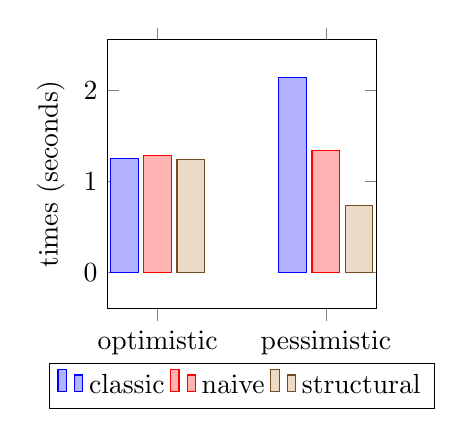
\begin{tikzpicture}
\begin{axis}[
    ybar, ymax = 2, ymin = 0.15,
    enlargelimits=0.3,
    width=5cm, height=5cm,
    legend style={at={(0.5,-0.2)},
      anchor=north,legend columns=-1},
    ylabel={times (seconds)},
    symbolic x coords={optimistic, pessimistic},
    xtick=data
    ]
\addplot coordinates {(optimistic,1.254) (pessimistic,2.142)};
\addplot coordinates {(optimistic,1.282) (pessimistic,1.337)};
\addplot coordinates {(optimistic,1.236) (pessimistic,0.733)};
\legend{classic,naive,structural}
\end{axis}
\end{tikzpicture}
 \captionof{figure}{revers$^o$ forward evaluation \\ for a list with a length of 90}
  \label{fair:plot-reverso}
\end{minipage}%
\begin{minipage}{.5\textwidth}
  \centering
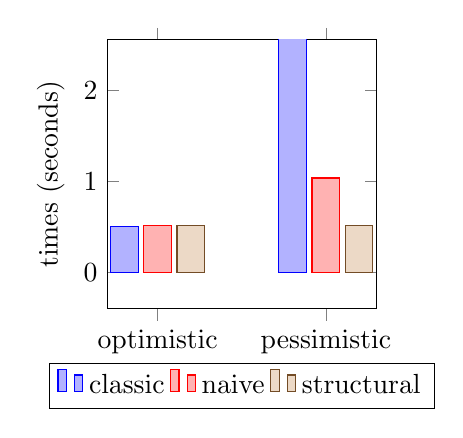
\begin{tikzpicture}
\begin{axis}[
    ybar, ymax = 2, ymin = 0.15,
    enlargelimits=0.3,
    width=5cm, height=5cm,
    legend style={at={(0.5,-0.2)},
      anchor=north,legend columns=-1},
    ylabel={times (seconds)},
    symbolic x coords={optimistic, pessimistic},
    xtick=data
    ]
\addplot coordinates {(optimistic,0.504) (pessimistic,300)};
\addplot coordinates {(optimistic,0.508) (pessimistic,1.035)};
\addplot coordinates {(optimistic,0.513) (pessimistic,0.513)};
\legend{classic,naive,structural}
\end{axis}
\end{tikzpicture}
 \captionof{figure}{sort$^o$ forward evaluation \\ for a list with a length of 5}
\label{fair:plot-sorto}
\end{minipage}
\end{figure*}

\begin{figure*}
\centering
\begin{minipage}{.5\textwidth}
  \centering
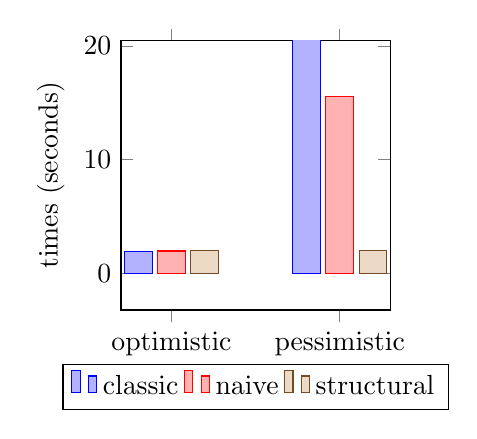
\begin{tikzpicture}
\begin{axis}[
    ybar, ymax = 16, ymin = 1.2,
    enlargelimits=0.3,
    width=5cm, height=5cm,
    legend style={at={(0.5,-0.2)},
      anchor=north,legend columns=-1},
    ylabel={times (seconds)},
    symbolic x coords={optimistic, pessimistic},
    xtick=data
    ]
\addplot coordinates {(optimistic,1.909) (pessimistic,300)};
\addplot coordinates {(optimistic,1.945) (pessimistic,15.516)};
\addplot coordinates {(optimistic,1.980) (pessimistic,1.978)};
\legend{classic,naive,structural}
\end{axis}
\end{tikzpicture}
 \captionof{figure}{``The Tower of Hanoi'' \\ solver evaluation}
\label{fair:plot-hanoi}
\end{minipage}%
\begin{minipage}{.5\textwidth}
  \centering
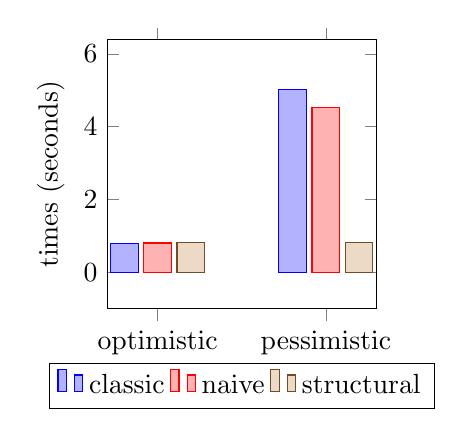
\begin{tikzpicture}
\begin{axis}[
    ybar, ymax = 5, ymin = 0.375,
    enlargelimits=0.3,
    width=5cm, height=5cm,
    legend style={at={(0.5,-0.2)},
      anchor=north,legend columns=-1},
    ylabel={times (seconds)},
    symbolic x coords={optimistic, pessimistic},
    xtick=data
    ]
\addplot coordinates {(optimistic,0.783) (pessimistic,5.019)};
\addplot coordinates {(optimistic,0.801) (pessimistic,4.522)};
\addplot coordinates {(optimistic,0.812) (pessimistic,0.817)};
\legend{classic,naive,structural}
\end{axis}
\end{tikzpicture}
 \captionof{figure}{``Bridge and torch problem'' \\ solver evaluation}
\label{fair:plot-bridge}
\end{minipage}
\end{figure*}

Now we will discuss evaluation. Целью эвалюации является выявления влияния порядка конъюнктов на эффективность трех различных семантик.

Первая семантика с предикатом $pred_{\mbox{\lstinline{true}}}$ близка к классическим реализациям \mk. В дальнейшем будем называть её {\bf left-biased}.

Вторая семантика с предикатом $pred_N$ соответсвует равномерному вычислению всех конъюнктов. Эту семантику будем назвать {\bf naive}.

Третья семантика с предикатом $pred_{\leq_{sr}}$ вычисляет структурно-рекурсивные конъюнкты, пока убывают структурно-рекурсивные аргументы. Её будем называть {\bf structural}.

For evaluation we've chosen two simple programs (list reversing and list sorting) and three more complicated (the ``Hanoi Towers''\footnote{\url{https://en.wikipedia.org/wiki/Tower_of_Hanoi}} solver, the
``Bridge and torch problem''\footnote{\url{https://en.wikipedia.org/wiki/Bridge_and_torch_problem}} solver and ``Water pouring puzzle''\footnote{\url{https://en.wikipedia.org/wiki/Water_pouring_puzzle}} solver).
% Для каждой программы мы сделали две версии. Оптимистичная версия --- это программа, в которой мы вручную подобрали оптимальный порядок конъюнктов и пессиместичная версия --- программа с неоптимальным порядком конъюнктов. В последующих диаграммах и таблице указаны средние значения 10 запусков тестов. Также для наивной равномерной конъюнкции мы подобрали количество разверток вручную. Для равномерной конъюнкции, основанной на структурной рекурсии, N было фиксировано и равно 100.
Each program was written in two versions: ``optimistic'' (with the order of important conjuncts set to provide the best performance) and ``pessimistic'' (with the order of important
conjuncts set to provide the worst performance). Also we evaluated list reversing and list sorting in both directions. In the case of the list reversing, queries \lstinline{(revers$^o$ [1;2;3] q)} and \lstinline{(revers$^o$ q [1;2;3])}\! will give the same answer \lstinline{q = [3;2;1]} but the ``optimistic'' order of conjuncts is different for them. In the case of list sorting, queries \lstinline{(sort$^o$ [1;2;3] q)} and \lstinline{(sort$^o$ q [1;2;3])} will give different answers. The first one gives sorted list \lstinline{q = [1;2;3]}, the second one gives all permutations of list \lstinline{[1;2;3]}\!\!. 

All benchmarks were run ten times, and the average time was taken. For the naive  semantics we cherry-picked the best value of unfolding bound manually. Structural arguments for each relations were detected automatically.

% На изображениях 12-15 представлены результаты апробации в виде столбцовых диаграмм. В оптимистичном случае результаты схожи для всех семантик. В пессиместичном случае время работы напрпавленной конъюнкции резко возрастает, время работы наивной равномерной конъюнкции также ворзрастает, но не так сильно. Равномерная конъюнкция, основанная на структурной рекурсии, демострирует схожую эффективность в сравнении с оптимистичным случаем.
Fig.~\ref{fair:plot-reverso}-\ref{fair:plot-bridge} show the results of evaluation in the form of bar charts. In the optimistic case, the results are similar for all semantics.
In the pessimistic case the evaluation time of the directed conjunction rapidly increases, the evaluation time of the naive fair conjunction also increases, but not so much.
The fair semantics based on structural recursion demonstrates a similar efficiency as in the optimistic case.

\begin{figure*} %[h!]
  \small
  \centering
  \begin{tabular}{ c | c | c | c | c | c | c | c }
    \multirow{2}{*}{relation} & \multirow{2}{*}{size} & 
    \multicolumn{2}{c}{left-biased semantics} &
    \multicolumn{2}{c}{naive semantics} &
    \multicolumn{2}{c}{structural semantics} \\
    \cline{3-8}
    & & optimistic & pessimistic & optimistic & pessimistic & optimistic & pessimistic  \\ 
    \hline
    \multirow{3}{*}{\begin{tabular}{c} forward \\ revers$^o$ \end{tabular}}
                 & 30   & 0.527 & 0.587  & 0.532 & 0.595   & 0.539 & 0.532 \\
                 & 60   & 0.639 & 0.947  & 0.643 & 0.790   & 0.657 & 0.577 \\
                 & 90   & 1.254 & 2.142  & 1.282 & 1.337   & 1.236 & 0.733 \\
    \hline
    \multirow{3}{*}{\begin{tabular}{c} backward \\ revers$^o$ \end{tabular}}
                 & 30   & 0.531 & 0.579  & 0.547 & 0.570  & 0.553 & 0.563 \\
                 & 60   & 0.655 & 0.875  & 0.667 & 0.812  & 0.668 & 0.681 \\
                 & 90   & 1.316 & 1.813  & 1.327 & 1.503  & 1.360 & 1.359 \\
    \hline
    \multirow{5}{*}{\begin{tabular}{c} forward \\ sort$^o$ \end{tabular}}
                 & 3    & 0.467 & 0.503  & 0.474 & 0.481  & 0.472 & 0.479 \\
                 & 4    & 0.484 & 4.679  & 0.485 & 0.493  & 0.490 & 0.488 \\
                 & 5    & 0.504 & $>$300 & 0.508 & 1.035  & 0.513 & 0.513 \\
                 & 6    & 0.526 & $>$300 & 0.237 & 14.369 & 0.544 & 0.547 \\
                 & 30   & 1.915 & $>$300 & 1.936 & $>$300 & 1.983 & 1.987 \\
    \hline
    \multirow{4}{*}{\begin{tabular}{c} backward \\ sort$^o$ \end{tabular}}
                 & 3    & 0.518 &  0.519 & 0.518 & 0.521  & 0.520 & 0.521 \\
                 & 4    & 0.533 &  0.856 & 0.534 & 0.540  & 0.534 & 0.537 \\
                 & 5    & 0.680 & 93.914 & 0.713 & 1.528  & 0.718 & 0.714 \\
                 & 6    & 2.931 & $>$300 & 2.947 & 59.647 & 2.938 & 2.936 \\
    \hline
    hanoi$^o$    & -    & 1.909 & $>$300 & 1.945 & 15.516 & 1.980 & 1.978 \\
    \hline
    bridge$^o$   & -    & 0.783 & 5.019  & 0.801 & 4.522  & 0.812 & 0.817 \\
    \hline
    water$^o$    & -    & 3.513 & $>$300 & 3.518 & $>$300 & 3.538 & 3.771

  \end{tabular}
  \caption{The results of evaluation: running times of benchmarks in seconds}
  \label{fair:evaluation-table}
\end{figure*}

% Более подробно результаты представлены на изображении 16. Можно заметить, что время работы программы sorto в пессиместичном случае очень быстро растет с увеличением длины списка для направленной конъюнкции и наивной равномерной. В случае с равномерной конъюнкцией, основанной на структурной рекурсии, пессиместичный случай растет сопостовимо с оптимистичным.
The results are presented in more detail in Fig.~\ref{fair:evaluation-table}. ``Hanoi Towers'' solver has name \lstinline{hanoi$^o$}, ``Bridge and torch problem'' solver has name \lstinline{bridge$^o$} and ``Water pouring puzzle'' solver has name \lstinline{water$^o$}. We can conclude that forward and backward \lstinline{sort$^o$} runtime in the pessimistic case increases very rapidly with increasing the list length for left-biased and naive fair semantics. In the case of the fair semantics based on structural recursion the running time in pessimistic case increases on a par with that in the optimistic one. Also the solver \lstinline{water$^o$} very slow in the pessimistic case for left-biased and naive fair. However, fair conjunction based on structural recursion pessimistic case is no different from an optimistic case.


% Подводя итог, равномерная конъюнкция, основанная на структурной рекурсии сопоставима по эффективности с направленной конъюнкцией. Более того, это конъюнкция слабо зависит от порядка конъюнктов.
To summarize, the fair semantics based on structural recursion does not introduce any essential overhead in comparison with left-biased semantics in an optimistic case. At the same time it
weakly depends on the order of the conjuncts, and thus demonstrates much better performance in the pessimistic case.

% \section{Conclusion}
\label{conclusion}

We presented an approach for converting typed functional programs into relations. Relational conversion 
in many cases allows us to avoid tedious recoding of functional specifications into relational form and to 
concentrate on writing relational specifications only when their reconstruction from functions is impossible or 
undesirable. Our implementation works for the subset of OCaml; we evaluated it for a number of interesting 
examples and acquired some new relational solutions.

There is a number of directions for future research. First, a performance evaluation is desirable~--- at
present time we do not know, what slowdown factor is. Another problem is a development of an approach to
prove complete correctness (or refute this claim).


%%
%% The acknowledgments section is defined using the "acks" environment
%% (and NOT an unnumbered section). This ensures the proper
%% identification of the section in the article metadata, and the
%% consistent spelling of the heading.
%%\begin{acks}

%%\end{acks}

%%
%% The next two lines define the bibliography style to be used, and
%% the bibliography file.
% \bibliographystyle{splncs04}
% \bibliography{main}

%%
%% If your work has an appendix, this is the place to put it.
\appendix

% \section{Definitions of the evaluated relations}
\label{sec:examples_definitions}

Here are the definitions of the \mK relations we used for evaluation. Different queries to the same relation may require different orders in conjunctions.

\begin{enumerate}

\item Comparison of Peano numbers

\begin{minipage}{\linewidth}
Definition:

\begin{lstlisting}[basicstyle=\small]
   le$^o$ = fun x y ->
     (x === O) \/
     (fresh (x' y')
        (x === S(x')) /\
        (y === S(y')) /\
        (le$^o$ x' y')
     )
\end{lstlisting}
\end{minipage}

\begin{minipage}{\linewidth}
For queries:

\begin{itemize}
\item[-] \lstinline{le$^o$ $\overline{n}$ $\overline{m}$}

\item[-] \lstinline{le$^o$ $x^?$ $\overline{m}$}

\item[-] \lstinline{le$^o$ $\overline{n}$ $y^?$}
\end{itemize}
\end{minipage}


\item Sum of Peano numbers

\begin{minipage}{\linewidth}
Definition:

\begin{lstlisting}[basicstyle=\small]
   plus$^o$ = fun x y r ->
     ((x === O) /\ (y === r)) \/
     (fresh (x' r')
        (x === S(x')) /\
        (r === S(r')) /\
        (plus$^o$ x' y r')
     )
\end{lstlisting}
\end{minipage}

\begin{minipage}{\linewidth}
For queries:

\begin{itemize}
\item[-] \lstinline{plus$^o$ $\overline{n}$ $\overline{m}$ $r^?$}

\item[-] \lstinline{plus$^o$ $\overline{n}$ $y^?$ $\overline{k}$}

\item[-] \lstinline{plus$^o$ $x^?$ $y^?$ $\overline{k}$}
\end{itemize}
\end{minipage}


\item Product of Peano numbers

\begin{minipage}{\linewidth}
Definition \#1:

\begin{lstlisting}[basicstyle=\small]
   mult$^o$ = fun x y r ->
     ((x === O) /\ (r === O)) \/
     (fresh (x' r')
        (x === S(x')) /\
        (mult$^o$ x' y r') /\
        (plus$^o$ r' y r)
     )
\end{lstlisting}
\end{minipage}

\begin{minipage}{\linewidth}
For query:

\begin{itemize}
\item[-] \lstinline{mult$^o$ $\overline{n}$ $\overline{m}$ $r^?$}
\end{itemize}
\end{minipage}

\begin{minipage}{\linewidth}
Definition \#2:

\begin{lstlisting}[basicstyle=\small]
   mult$^o$ = fun x y r ->
     ((x === O) /\ (r === O)) \/
     (fresh (x' r')
        (x === S(x')) /\
        (plus$^o$ r' y r) /\
        (mult$^o$ x' y r')
     )
\end{lstlisting}
\end{minipage}

\begin{minipage}{\linewidth}
For queries:

\begin{itemize}
\item[-] \lstinline{mult$^o$ $x^?$ $\overline{m + 1}$ $\overline{k}$}

\item[-] \lstinline{mult$^o$ S($x^?$) S($y^?$) $\overline{k}$}
\end{itemize}
\end{minipage}


\item Length of a list

\begin{minipage}{\linewidth}
Definition \#1:

\begin{lstlisting}[basicstyle=\small]
   length$_d^o$ = fun a r ->
     ((a === Nil) /\ (x === O)) \/
     (fresh (h t r')
        (a === Cons(h, t)) /\
        (length$_d^o$ t r') /\
        (r === S(r'))
     )
\end{lstlisting}
\end{minipage}

\begin{minipage}{\linewidth}
For query:

\begin{itemize}
\item[-] \lstinline{length$_d^o$ $\overline{l}$ $r^?$}
\end{itemize}
\end{minipage}

\begin{minipage}{\linewidth}
Definition \#2:

\begin{lstlisting}[basicstyle=\small]
   length$^o$ = fun a r ->
     ((a === Nil) /\ (x === O)) \/
     (fresh (h t r')
        (a === Cons(h, t)) /\
        (r === S(r')) /\
        (length$^o$ t r')
     )
\end{lstlisting}
\end{minipage}

\begin{minipage}{\linewidth}
For queries:

\begin{itemize}
\item[-] \lstinline{length$^o$ $\overline{l}$ $r^?$}

\item[-] \lstinline{length$^o$ $a^?$ $\overline{n}$}
\end{itemize}
\end{minipage}


\item Incrementing all elements in a list

\begin{minipage}{\linewidth}
Definition:

\begin{lstlisting}[basicstyle=\small]
   incr_list$^o$ = fun a r ->
     ((a === Nil) /\ (r === Nil)) \/
     (fresh (h t tr)
        (a === Cons(h, t)) /\
        (r === Cons(S(h), tr)) /\
        (incr_list$^o$ t tr)
     )
\end{lstlisting}
\end{minipage}

\begin{minipage}{\linewidth}
For queries:

\begin{itemize}
\item[-] \lstinline{incr_list$^o$ $\overline{l}$ $r^?$}

\item[-] \lstinline{incr_list$^o$ $a^?$ $\overline{l}$}
\end{itemize}
\end{minipage}



\item Concatination of two lists

\begin{minipage}{\linewidth}
Definition:

\begin{lstlisting}[basicstyle=\small]
   append$^o$ = fun a b r ->
     ((a === Nil) /\ (b === r)) \/
     (fresh (h t tb)
        (a === Cons(h, t)) /\
        (r === Cons(h, tb)) /\
        (append$^o$ t b tb)
     )
\end{lstlisting}
\end{minipage}

\begin{minipage}{\linewidth}
For queries:

\begin{itemize}
\item[-] \lstinline{append$^o$ $\overline{l_1}$ $\overline{l_2}$ $r^?$}

\item[-] \lstinline{append$^o$ $a^?$ $b^?$ $\overline{l}$}
\end{itemize}
\end{minipage}


\item Inversion of a list

\begin{minipage}{\linewidth}
Definition \#1:

\begin{lstlisting}[basicstyle=\small]
   reverse$^o$ = fun a r ->
     ((a === Nil) /\ (r === Nil)) \/
     (fresh (h t tb)
        (a === Cons(h, t)) /\
        (reverse$^o$ t tr) /\
        (append$^o$ tr Cons(h, Nil) r)
     )
\end{lstlisting}
\end{minipage}

\begin{minipage}{\linewidth}
For query:

\begin{itemize}
\item[-] \lstinline{reverse$^o$ $\overline{l}$ $r^?$}
\end{itemize}
\end{minipage}
 
\begin{minipage}{\linewidth}
Definition \#2:

\begin{lstlisting}[basicstyle=\small]
   reverse$^o$ = fun a r ->
     ((a === Nil) /\ (r === Nil)) \/
     (fresh (h t tb)
        (a === Cons(h, t)) /\
        (append$^o$ tr Cons(h, Nil) r) /\
        (reverse$^o$ t tr)
     )
\end{lstlisting}
\end{minipage}

\begin{minipage}{\linewidth}
For query:

\begin{itemize}
\item[-] \lstinline{reverse$^o$ $a^?$ $\overline{l}$}
\end{itemize}
\end{minipage}

\end{enumerate} 

\end{document}
\endinput
%%
%% End of file `sample-acmlarge.tex'.
